\documentclass[a4paper,12pt,twoside]{memoir}

% Castellano
\usepackage[spanish,es-tabla]{babel}
\selectlanguage{spanish}
\usepackage[utf8]{inputenc}
\usepackage[T1]{fontenc}
\usepackage{lmodern} % scalable font
\usepackage{microtype}
\usepackage{placeins}

\RequirePackage{booktabs}
\RequirePackage[table]{xcolor}
\RequirePackage{xtab}
\RequirePackage{multirow}

% Links
\PassOptionsToPackage{hyphens}{url}\usepackage[colorlinks]{hyperref}
\hypersetup{
	allcolors = {red}
}

% Ecuaciones
\usepackage{amsmath}

% Rutas de fichero / paquete
\newcommand{\ruta}[1]{{\sffamily #1}}

% Párrafos
\nonzeroparskip

% Huérfanas y viudas
\widowpenalty100000
\clubpenalty100000

% Evitar solapes en el header
\nouppercaseheads

% Imagenes
\usepackage{graphicx}
\newcommand{\imagen}[2]{
	\begin{figure}[!h]
		\centering
		\includegraphics[width=0.9\textwidth]{#1}
		\caption{#2}\label{fig:#1}
	\end{figure}
	\FloatBarrier
}

\newcommand{\imagenflotante}[2]{
	\begin{figure}%[!h]
		\centering
		\includegraphics[width=0.9\textwidth]{#1}
		\caption{#2}\label{fig:#1}
	\end{figure}
}



% El comando \figura nos permite insertar figuras comodamente, y utilizando
% siempre el mismo formato. Los parametros son:
% 1 -> Porcentaje del ancho de página que ocupará la figura (de 0 a 1)
% 2 --> Fichero de la imagen
% 3 --> Texto a pie de imagen
% 4 --> Etiqueta (label) para referencias
% 5 --> Opciones que queramos pasarle al \includegraphics
% 6 --> Opciones de posicionamiento a pasarle a \begin{figure}
\newcommand{\figuraConPosicion}[6]{%
  \setlength{\anchoFloat}{#1\textwidth}%
  \addtolength{\anchoFloat}{-4\fboxsep}%
  \setlength{\anchoFigura}{\anchoFloat}%
  \begin{figure}[#6]
    \begin{center}%
      \Ovalbox{%
        \begin{minipage}{\anchoFloat}%
          \begin{center}%
            \includegraphics[width=\anchoFigura,#5]{#2}%
            \caption{#3}%
            \label{#4}%
          \end{center}%
        \end{minipage}
      }%
    \end{center}%
  \end{figure}%
}

%
% Comando para incluir imágenes en formato apaisado (sin marco).
\newcommand{\figuraApaisadaSinMarco}[5]{%
  \begin{figure}%
    \begin{center}%
    \includegraphics[angle=90,height=#1\textheight,#5]{#2}%
    \caption{#3}%
    \label{#4}%
    \end{center}%
  \end{figure}%
}
% Para las tablas
\newcommand{\otoprule}{\midrule [\heavyrulewidth]}
%
% Nuevo comando para tablas pequeñas (menos de una página).
\newcommand{\tablaSmall}[5]{%
 \begin{table}
  \begin{center}
   \rowcolors {2}{gray!35}{}
   \begin{tabular}{#2}
    \toprule
    #4
    \otoprule
    #5
    \bottomrule
   \end{tabular}
   \caption{#1}
   \label{tabla:#3}
  \end{center}
 \end{table}
}

%
%Para el float H de tablaSmallSinColores
\usepackage{float}

%
% Nuevo comando para tablas pequeñas (menos de una página).
\newcommand{\tablaSmallSinColores}[5]{%
 \begin{table}[H]
  \begin{center}
   \begin{tabular}{#2}
    \toprule
    #4
    \otoprule
    #5
    \bottomrule
   \end{tabular}
   \caption{#1}
   \label{tabla:#3}
  \end{center}
 \end{table}
}

\newcommand{\tablaApaisadaSmall}[5]{%
\begin{landscape}
  \begin{table}
   \begin{center}
    \rowcolors {2}{gray!35}{}
    \begin{tabular}{#2}
     \toprule
     #4
     \otoprule
     #5
     \bottomrule
    \end{tabular}
    \caption{#1}
    \label{tabla:#3}
   \end{center}
  \end{table}
\end{landscape}
}

%
% Nuevo comando para tablas grandes con cabecera y filas alternas coloreadas en gris.
\newcommand{\tabla}[6]{%
  \begin{center}
    \tablefirsthead{
      \toprule
      #5
      \otoprule
    }
    \tablehead{
      \multicolumn{#3}{l}{\small\sl continúa desde la página anterior}\\
      \toprule
      #5
      \otoprule
    }
    \tabletail{
      \hline
      \multicolumn{#3}{r}{\small\sl continúa en la página siguiente}\\
    }
    \tablelasttail{
      \hline
    }
    \bottomcaption{#1}
    \rowcolors {2}{gray!35}{}
    \begin{xtabular}{#2}
      #6
      \bottomrule
    \end{xtabular}
    \label{tabla:#4}
  \end{center}
}

%
% Nuevo comando para tablas grandes con cabecera.
\newcommand{\tablaSinColores}[6]{%
  \begin{center}
    \tablefirsthead{
      \toprule
      #5
      \otoprule
    }
    \tablehead{
      \multicolumn{#3}{l}{\small\sl continúa desde la página anterior}\\
      \toprule
      #5
      \otoprule
    }
    \tabletail{
      \hline
      \multicolumn{#3}{r}{\small\sl continúa en la página siguiente}\\
    }
    \tablelasttail{
      \hline
    }
    \bottomcaption{#1}
    \begin{xtabular}{#2}
      #6
      \bottomrule
    \end{xtabular}
    \label{tabla:#4}
  \end{center}
}

%
% Nuevo comando para tablas grandes sin cabecera.
\newcommand{\tablaSinCabecera}[5]{%
  \begin{center}
    \tablefirsthead{
      \toprule
    }
    \tablehead{
      \multicolumn{#3}{l}{\small\sl continúa desde la página anterior}\\
      \hline
    }
    \tabletail{
      \hline
      \multicolumn{#3}{r}{\small\sl continúa en la página siguiente}\\
    }
    \tablelasttail{
      \hline
    }
    \bottomcaption{#1}
  \begin{xtabular}{#2}
    #5
   \bottomrule
  \end{xtabular}
  \label{tabla:#4}
  \end{center}
}



\definecolor{cgoLight}{HTML}{EEEEEE}
\definecolor{cgoExtralight}{HTML}{FFFFFF}

%
% Nuevo comando para tablas grandes sin cabecera.
\newcommand{\tablaSinCabeceraConBandas}[5]{%
  \begin{center}
    \tablefirsthead{
      \toprule
    }
    \tablehead{
      \multicolumn{#3}{l}{\small\sl continúa desde la página anterior}\\
      \hline
    }
    \tabletail{
      \hline
      \multicolumn{#3}{r}{\small\sl continúa en la página siguiente}\\
    }
    \tablelasttail{
      \hline
    }
    \bottomcaption{#1}
    \rowcolors[]{1}{cgoExtralight}{cgoLight}

  \begin{xtabular}{#2}
    #5
   \bottomrule
  \end{xtabular}
  \label{tabla:#4}
  \end{center}
}




\graphicspath{ {./img/} }

% Capítulos
\chapterstyle{bianchi}
\newcommand{\capitulo}[2]{
	\setcounter{chapter}{#1}
	\setcounter{section}{0}
	\chapter*{#2}
	\addcontentsline{toc}{chapter}{#2}
	\markboth{#2}{#2}
}

% Apéndices
\renewcommand{\appendixname}{Apéndice}
\renewcommand*\cftappendixname{\appendixname}

\newcommand{\apendice}[1]{
	%\renewcommand{\thechapter}{A}
	\chapter{#1}
}

\renewcommand*\cftappendixname{\appendixname\ }

% Formato de portada
\makeatletter
\usepackage{xcolor}
\newcommand{\tutor}[1]{\def\@tutor{#1}}
\newcommand{\course}[1]{\def\@course{#1}}
\definecolor{cpardoBox}{HTML}{E6E6FF}
\def\maketitle{
  \null
  \thispagestyle{empty}
  % Cabecera ----------------
\noindent
\includegraphics[width=\textwidth]{cabecera}\vspace{1cm}%
  \vfill
  % Título proyecto y escudo informática ----------------
  \colorbox{cpardoBox}{%
    \begin{minipage}{.8\textwidth}
      \vspace{.5cm}\Large
      \begin{center}
      \textbf{TFG del Grado en Ingeniería Informática}\vspace{.6cm}\\
      \textbf{\LARGE\@title{}}
      \end{center}
      \vspace{.2cm}
    \end{minipage}

  }%
  \hfill\begin{minipage}{.20\textwidth}
    
\includegraphics[width=\textwidth]{escudoInfor}
  \end{minipage}
  \vfill
  % Datos de alumno, curso y tutores ------------------
  \begin{center}%
  {%
    \noindent\LARGE
    Presentado por \@author{}\\ 
    en Universidad de Burgos --- \@date{}\\
    Tutor: \@tutor{}\\
  }%
  \end{center}%
  \null
  \cleardoublepage
  }
\makeatother


% Datos de portada
\title{título del TFG \\Documentación Técnica}
\author{nombre alumno}
\tutor{nombre tutor}
\date{\today}

\begin{document}

\maketitle



\cleardoublepage



%%%%%%%%%%%%%%%%%%%%%%%%%%%%%%%%%%%%%%%%%%%%%%%%%%%%%%%%%%%%%%%%%%%%%%%%%%%%%%%%%%%%%%%%



\frontmatter


\clearpage

% Indices
\tableofcontents

\clearpage

\listoffigures

\clearpage

\listoftables

\clearpage

\mainmatter

\appendix

\apendice{Plan de Proyecto Software}

\section{Introducción}
Un plan de proyecto recoge la planificación temporal donde se resumen las divisiones de trabajo en periodos de tiempo y un estudio de viabilidad teniendo en cuenta las repercusiones tanto legales como económicas de dicho proyecto.

\section{Planificación temporal}
Para la planificación temporal se ha usado la plataforma GitHub en la que se ha intentado simular una metodología \textit{Scrum}, en la que las divisiones de tiempo para realizar una determinada función se conocen como \textit{Sprints}. La duración de los Sprints en este caso no era especificada, ya que no se tenían unos plazos obligatorios y algunos sprints duraban más de lo planeado y otros menos. Los primeros Sprints están resumidos en unas \textit{issues} de mayor tamaño ya que se centraban en realizar pruebas y generación del comienzo del proyecto.\newline
Dentro de la plataforma de GitHub se utilizó el tablero de Zen-hub para controlar mejor la inicialización y finalización de las \textit{issues}.\newline
El enlace GitHub del repositorio del presente trabajo puede encontrarse en:\newline \url{https://github.com/jgo0038/TFG-Reserva-aulas-informatica} \newline

\subsection{Sprint 0 - 24/02/2020 - 27/02/2020}
Primer sprint en el que se inicia el proyecto, realmente comienza antes el proyecto y la investigación pero hasta entonces no se crea el GitHub. Las tareas en este sprint estaban destinadas a la investigación y la preparación para el proyecto:
\begin{itemize}
    \item Elegir los programas a utilizar. 
	\item Crear un repositorio en GitHub.
    \item Generar el entorno virtual de trabajo.
    \item Registrar la aplicación en Azure Active Directory para obtener un identificador de la aplicación.
	\item Implementación una primera versión simple del login en nuestra web app.
	\item Empezar a manejar Overleaf para la documentación el LaTex.
	\item Investigar sobre el uso de la API de Outlook para Flask.
\end{itemize}
Una vez se registró la app en Azure, el objetivo principal era poder iniciar sesión en Outlook con los códigos recibidos, utilizando un repositorio de GitHub como \href{https://github.com/brysontyrrell/Office-365-Flask-App}{ayuda}\cite{loginO365}.
Resaltar que aquí creo la primera rama donde se subieron estos primeros pasos del proyecto.
\subsection{Sprint 1 - 27/02/2020 - 08/03/2020}
En este sprint solamente hubo especificada una tarea, que engloba trabajar con la API y empezar a enviar y recibir datos para conocer su funcionamiento. Ya conociendo la forma en la que iba a trabajar y los requisitos que había que conseguir, se comenzó a hacer pruebas sobre la API solucionando los primeros errores y consiguiendo los primeros avances.\newline
Una vez estaba iniciada la sesión de Outlook el objetivo de este Sprint era leer y modificar eventos del calendario de la sesión. Se sube esto a nueva nueva rama, que permite, a parte del inicio de sesión ya comentado en el Sprint 0, la funcionalidad de poder recoger eventos del calendario principal del usuario que ha iniciado sesión en la web app.

\subsection{Sprint 2 - 08/03/2020 - 05/04/2020}
Los objetivos principales en este sprint fueron los siguientes:
\begin{itemize}
    \item Investigar y comenzar a trabajar con los calendarios compartidos de Outlook.
    \item Comenzar a trabajar con la base de datos local de MySQL.
    \item Investigar sobre la seguridad de la aplicación.
\end{itemize}
En este Sprint, la tarea de investigar la seguridad era secundaria y no corría prisa de momento, por lo que se relegó a mirarlo más tarde cuando tuviera más funcionalidad y páginas creadas. La tarea principal era el trabajo con los calendarios compartidos, en concreto se buscaba poder crear eventos en calendarios compartidos, que son los que hacen la función de albergar los eventos de cada aula.

\subsection{Sprint 3 - 26/03/2020 - 15/04/2020}
Los objetivos que abordamos en este Sprint se centrar en añadir funcionalidades a la aplicación y estudiar el despliegue:
\begin{itemize}
    \item Controlar el solapamiento de horas de los eventos en los calendarios ya que no lo realiza Outlook.
    \item Añadir una página en la que se puedan ver los eventos que hay creados en un determinado calendario.
    \item Estudiar las posibilidades que hay para desplegar la web app. Se opta por utilizar Azure.
\end{itemize}
Este Sprint se fue compaginando con el anterior, ya que la tarea de investigar sobre la seguridad de la aplicación había quedado pendiente.
\subsection{Sprint 4 - 05/04/2020 - 27/04/2020}
Este Sprint tenía como objetivos principales:
\begin{itemize}
    \item Controlar que funcione en un entorno multiusuario, que no se pueda reservar a la vez el mismo aula.
    \item Crear el primer modelo de las tablas y relaciones en la base de datos local.
    \item Comprobar que las fechas de inicio y fin coincidan en una reserva simple.
    \item Ofrecer al cliente una opción para elegir de qué calendario quiere ver las horas reservadas de entre aquellos de los que es responsable.
\end{itemize}
Este Sprint se da por cerrado pese a haber quedado una tarea abierta (sincronizar la web app con la base de datos, de modo que borre los eventos de la base de datos local y los vuelva a guardar recuperándolos directamente desde Outlook, como solución a algún problema o corrupción de los datos de la base de datos), esta tarea fue desestimada en una reunión posterior. La base de datos y los calendarios de Outlook siempre tienen que estar sincronizados, compartiendo los mismos datos en ambos sitios, de forma que si se borra un evento del calendario, también se borre el correspondiente en la base de datos. Si esto fallara, más adelante no se podrían realizar reservas en fechas que en realidad deberían de estar libres.
\subsection{Sprint 5 - 17/04/2020 - 07/05/2020}
Los objetivos que voy a abordar en este Sprint son los siguientes:
\begin{itemize}
    \item Realizar un cambio en una relación de la base de datos, permite albergar mas de un propietario a un aula.
    \item Crear el servidor de Azure database, se crea en lenguaje SQL y sin servidor, para reducir el coste al mínimo.
    \item Subir la base de datos local al servidor de Azure database creado y adaptar el lenguaje al SQL server.
    \item Conectar la base de datos subida a Azure con nuestra web app, se realiza mediante pyodbc.
    \item Organizar el proyecto según el estandar establecido por Microsoft y VSCode para poder subir facilmente a Azure.
    \item Desplegar la aplicación en Azure.
    \item Primera asignación y restricción de acceso a páginas según la cuenta que acceda.
\end{itemize}

\subsection{Sprint 6 - 07/05/2020 - 15/06/2020}
Este Sprint se centra en mejorar partes del código ya existentes y facilitar la reserva de las aulas, concretamente los objetivos fueron:
\begin{itemize}
    \item Solucionar los errores de los formularios, que no se muestran por pantalla correctamente.
    \item Añadir unos filtros antes de reservar el aula, limitando las aulas que se muestran. Añadir también un campo para el nombre del profesor que lo reserva.
    \item Crear una nueva página en la que el administrador pueda crear nuevas aulas.
    \item Crear una nueva página desde la que se pueda ver la información de cada aula.
    \item En la página de la información, permitir el modificar los datos de las aulas.
    \item Restringir los datos que se pueden introducir al modificar aulas en campos como propietario, edificio o tipo de aula.
    \item En la página de la información, permitir una opción para borrar las aulas.
    \item Añadir las opciones de reserva múltiple (reservar más de un día seguido a la misma hora) y de reserva periódica (reservar un día a la semana a la misma hora durante el tiempo que se quiera ).
    \item Crear una pagina de auditoría para el usuario administrador, desde la que puedan ver las altas, bajas y modificaciones que se realizan sobre los eventos.
\end{itemize}
Comentar que se actualiza también la base de datos, aplicando la actualización y borrado en cascada.
La fecha de finalización se alargó tanto ya que la tarea de la tabla de auditorías quedó pospuesta, de forma que si quedaba tiempo al final para realizarla se haría, por ello fue terminada el 15/06.

\subsection{Sprint 7 - 20/05/2020 - 17/06/2020}
El Sprint 7 se centra en volver a introducir el código con el que se ha estado trabajando en Azure e ir añadiendo la documentación al proyecto, para ello se fijan estos objetivos:
\begin{itemize}
    \item Actualizar el repositorio, añadiendo todo tal cual está con los cambios subidos a Azure.
    \item Añadir la carpeta de documentación siguiendo la plantilla proporcionada.
    \item Agregar la documentación realizada hasta entonces.
    \item Añadir los casos de uso.
\end{itemize}

\subsection{Sprint 8 - 26/05/2020 - 17/06/2020}
Este Sprint se centra en tareas más cortas y más visibles, dando estilos a la página y sus elementos y añadiendo funciones para mejorar el funcionamiento. Las tareas más destacables son las siguientes:
\begin{itemize}
    \item Añadir botón que permita ver las horas ocupadas del aula a reservar.
    \item Añadir cabeceras a las páginas.
    \item Añadir un campo nuevo de 'nº de ordenadores' a las aulas, si no tiene ordenadores se indicará con un 0. Establecer este campo como filtro al reservar aula también.
    \item Añadir campo de correo electrónico del nombre del profesor al que se reserva el aula y enviarle un mensaje cuando la reserva se realice.
    \item Representar los privilegios de cada usuario en los botones, de forma que se bloquee si no tiene permiso para esa función.
    \item Mostrar mensaje al modificar el campo propietario recordando al administrador que tiene que darle los permisos al nuevo propietario manualmente desde el calendario de Outlook.
    \item Aplicar estilos a los elementos de la página.
    \item Crear la barra de navegación.
    \item Implementar el cierre de sesión.
    \item Diseñar la página de inicio de la aplicación.
    \item Diseñar la página principal al iniciar sesión.
    \item Crear la barra de navegación en un fichero aparte del que puedan heredar dicho código.
\end{itemize}
Anótese que los filtros de búsqueda de capacidad y nº de ordenadores en la página de realizar reserva se atienen al mínimo buscado, no es un búsqueda exacta de esas características, sino se limitaría demasiado.

\subsection{Sprint 9 - 08/06/2020 - 26/06/2020}
Este sprint se crea después de una corrección completa del proyecto por el tutor. Anotando los fallos encontrados, las mejoras a realizar y funcionalidades pendientes:
\begin{itemize}
    \item Mejorar la página de eventos, dejando más claro su funcionamiento y eliminando el apartado de los filtros, convirtiéndolo en un mismo formulario.
    \item Añadir función de modificar eventos.
    \item Añadir función de borrar eventos.
    \item Arreglar el envío de mensaje al realizar una reserva.
    \item Añadir posibilidad de que el administrador añada propietarios nuevos.
    \item Añadir posibilidad al administrador de modificar los propietarios existentes.
    \item Arreglar la búsqueda de la página de reservas.
    \item Añadir un botón al consultar los eventos que permita mostrar y ocultar los eventos pasados.
    \item Arreglar los casos de uso tras la revisión realizada por el tutor.
    \item Rediseñar la página de consulta de eventos, para que sea mas intuitiva y más útil.
    \item Añadir una funcionalidad para que se puedan borrar más de un evento a la vez.
    \item Arreglar o mejorar pequeños detalles.
\end{itemize}

\subsection{Sprint 10 - 18/06/2020 - 26/06/2020 }
Realizar los últimos archivos de documentación que quedan por rellenar y completar o modificar algunos ya realizados.
\begin{itemize}
    \item Realizar el apartado de trabajos relacionados.
    \item Realizar el manual del programador.
    \item Realizar el manual del usuario.
    \item Mejoras sobre la documentación tras revisión del tutor.
\end{itemize}
\subsection{Sprint 11 - 01/07/2020 - 16/07/2020 }
Completar la aplicación con mejoras visuales y de funcionalidad.
\begin{itemize}
    \item Añadir una opción de seleccionar todos los eventos de la tabla para borrarlos a la vez.
    \item Añadir un filtro de fechas para la búsqueda en la tabla de auditorías.
    \item Permitir acceder a la aplicación como un usuario sin registrar y poder realizar la consulta de aulas y de eventos.
    \item Mejorar la pantalla de ayuda del mensaje al realizar acciones sobre el propietario.
    \item Permitir una búsqueda de un rango de fechas en la visualización de los eventos.
    \item Añadir más información al email que se envía al crear una reserva.
    \item Arreglar la reserva periódica que fallaba en algunos casos concretos.
    \item Actualizar la suscripción de Azure al haberse finalizado la de estudiante.
    \item Arreglar la consultas para ver las horas reservadas.
    \item Arreglar la modificación de la reserva al cambiar la hora a una que coincide con esta misma reserva.
\end{itemize}
\section{Estudio de viabilidad}
En esta sección trataré la viabilidad del proyecto, tanto en el ámbito económico como legal.
\subsection{Viabilidad económica}
En este apartado trataré de alcanzar el precio total del proyecto si fuera desarrollado en una empresa o comprado por alguien.\newline
\subsubsection{Coste de personal}
Para realizar este proyecto, se ha necesitado un desarrollador de aplicaciones web para lograrlo. Por lo tanto, el coste del personal se estima en lo siguiente:\newline
\subsubsection{Desarrollador}
Suponiendo que acaba de comenzar su carrera como desarrollador web, el sueldo medio está entre 17.000 y 22.000. Suponemos un término medio de 20.000 para realizar los cálculos. Lo que supone a la empresa: 
    \begin{equation}
        20.000 \div 12 = 1667 bruto
    \end{equation}
    El trabajo se ha realizado de finales de Febrero a finales de Junio, lo que suponen 4 meses.
\tablaSmallSinColores{Coste Desarrollador}{p{6.4cm} p{2.15cm} p{8cm}}{costedesarrollador}{
  \multicolumn{1}{p{4.5cm}}{\textbf{Concepto}} & \textbf{Coste mensual{}}\\
 }
 {
  Salario mensual  & \multicolumn{1}{r}{1667}\\\hline
  Costes seguridad social (23,60\%) & \multicolumn{1}{r}{393}\\\hline
  Cotización por formación profesional (0'6\%) &
  \multicolumn{1}{r}{10}\\\hline
  \textbf{Coste total (4 meses)}  & \multicolumn{1}{r}{7071}\\\hline
  }



\subsubsection{Coste hardware}
El coste del hardware utilizado se reduce al coste del portátil usado para desarrollar el proyecto. El precio del ordenador portátil (Asus X541U) con IVA fuese de 600, el desarrollo se estima que durará 4 meses, y se supone una amortización de este mismo de 4 años. Por lo que el precio usado del portátil sería:\newline
\begin{equation}
    (600 \div(12 * 4))* 4 = 50
\end{equation}

\subsubsection{Coste del despliegue}
El despliegue se ha realizado en Azure, donde se han ido realizando llamadas a la base de datos y ejecutando la aplicación subida. Esto se realizó con una suscripción a la cuenta de estudiante de Azure en la que se proporciona 100USD gratuitos. El uso de esta aplicación web para pruebas y mejoras ha supuesto un gasto de 100USD de los 100 disponibles, por lo que se agotó la suscripción de estudiante y hubo que mejorarla a una suscripción de pago por uso. Por esta razón el gasto en este caso ha sido 110USD, teniendo en cuenta que ha sido durante 4 meses, el coste mensual se estima en 27.5USD. Pero este coste se aplicaría a una empresa durante este período de desarrollo. Si se quisiera mantener después aumentaría dependiendo del uso que se hiciera de esta aplicación y del plan de pago que se eligiera. Esta cantidad de 110USD pasado a euros a fecha de 17/07/2020 hace un total de 96.28 euros.

\subsubsection{Coste total}
\tablaSmallSinColores{Coste Total}{p{6.4cm} p{2.15cm} p{8cm}}{costetotal}{
  \multicolumn{1}{p{4.5cm}}{\textbf{Concepto}} & \textbf{Coste{}}\\
 }
 {
  Coste desarrollador  & \multicolumn{1}{r}{7071}\\
  Hardware & \multicolumn{1}{r}{50}\\\hline
  Despliegue & \multicolumn{1}{r}{96.28}\\\hline
  Internet & \multicolumn{1}{r}{26*4} \\\hline
  \textbf{Coste total (4 meses)}  & \multicolumn{1}{r}{7321.28}\\\hline
  }


\subsection{Viabilidad legal}

En cuanto al código, todo lo utilizado en este proyecto es de libre distribución y dominio público. Se ha utilizado Flask y librerías de Python públicas.\newline
En cuanto a los programas utilizados, todos son públicos también.

\tablaSmallSinColores{Dependencias del proyecto.}{l c}{dependencias}
{ \multicolumn{1}{l}{\textbf{Dependencia}} & \textbf{Licencia}\\}{ 
astroid & LGPL\\\hline
click & BSD\\\hline
colorama & BSD\\\hline
distlib & Python Software Foundation License\\\hline
dominate  & LGPLv3\\\hline
filelock  & Public Domain\\\hline
Flask  & BSD\\\hline
Flask-Bootstrap & BSD\\\hline
Flask-SQLAlchemy  & BSD\\\hline
Flask-WTF  & BSD\\\hline
importlib-metadata  & Apache Software License\\\hline
importlib-resources  & Apache Software License\\\hline
isort   & MIT\\\hline
itsdangerous   & BSD\\\hline
Jinja2   & BSD\\\hline
MarkupSafe   & BSD\\\hline
mysqlclient   & GPL\\\hline
pylint   & GPL\\\hline
pyodbc  & MIT\\\hline
requests   & Apache 2\\\hline
six   & MIT\\\hline
SQLAlchemy  & MIT\\\hline
virtualenv   & MIT\\\hline
visitor  & MIT\\\hline
Werkzeug  & BSD\\\hline
wrapt  & BSD\\\hline
WTForms   & BSD\\\hline
zipp   & MIT\\\hline

}

Una vez se han visto las licencias a las que están sometidas las dependencias del proyecto, se ha seguido las recomendaciones de \cite{licencias} para determinar que este proyecto está bajo la licencia GPL-3.0, ya que es la última versión de la licencia GPL sobre software libre con \textit{copyleft}, lo que permite que todas las versiones sean libres.
\apendice{Especificación de Requisitos}

\section{Introducción}

\section{Objetivos generales}

\section{Catalogo de requisitos}

\section{Especificación de requisitos}



\apendice{Especificación de diseño}

\section{Introducción}
En esta sección será descrito el diseño que se ha llevado a cabo en la aplicación, especificando como se han resuelto los objetivos mas relevantes. En concreto, en los siguientes apartados se definirán los datos que maneja la aplicación, los detalles procedimentales y el diseño arquitectónico.
\section{Diseño de datos}
En este apartado se explicarán el conjunto de datos que se utilizan en la aplicación y mostraré el diagrama entidad relación seguido en la aplicación para mostrar la conexión entre los conjuntos de datos.

\imagen{DiagramaER.png}{Diagrama Entidad/Relación del proyecto.}

\subsection{Edificios}
Agrupación de aulas que se encuentran en el mismo edificio. En nuestra aplicación se representa como un grupo de calendarios compartido de Outlook gestionados por el administrador.

\subsection{Aulas}
Entidad sobre la que se realizan las reservas, se ubican en un edificio y podrían tener más de un propietario asignado. En nuestra aplicación las aulas se representan como calendarios compartidos dentro de un grupo de calendarios (edificio) sobre los que se va a poder realizar una reserva.

\subsection{Reservas}
Fecha del calendario entre unas horas específicas que se reserva para un usuario, la reserva es única en cada calendario. En nuestra aplicación se representa como un evento creado dentro de un aula (calendario) especificado, al ser único no puede haber más de un evento (reserva) en el mismo calendario a la misma hora o en horas que se solapen, pero sí puede haber eventos con el mismo nombre.

\subsection{Propietarios}
Se utiliza para designar indistintamente a un centro o a un departamento que podrá realizar modificaciones sobre sus aulas asignadas. Cada propietario tendrá un único responsable, éste será un usuario registrado con Outlook que tenga permisos para realizar reservas y modificaciones sobre las reservas de aulas de las que son propietarios.

\subsection{Auditoría}
Tabla en la que se registrarán las altas, bajas y modificaciones de las reservas. Además se guardará información sobre dichas alteraciones en la reserva, será solo visible para el administrador.

\section{Diseño procedimental}
En este apartado se mostrarán los diagramas de secuencias de las interacciones más destacadas de la aplicación.

\imagen{Diagrama_secuencias.png}{Diagrama de secuencias de las tareas principales del proyecto.}
En el diagrama superior, se puede apreciar las interacciones que se pueden realizar desde la aplicación, aquí cabe resaltar que las transacciones de modificar/borrar y crear reservas trabajan sobre la base de datos y sobre los calendarios de Outlook, por lo que se sincronizan ambas cada vez que se realiza una acción de las mencionadas.
\section{Diseño arquitectónico}
En este apartado se mostrará como está estructurado el código de la aplicación. Al tratarse de una web app se distinguen tres grandes agrupaciones siguiendo el patrón MVC (Modelo - Vista - Controlador). Según este patrón vamos a distinguir en la estructura de los datos el modelo de datos, la interfaz y la lógica de la aplicación en el controlador.\newline
En este proyecto en concreto, podemos distinguir los siguientes tipos de ficheros que realizan operaciones con distintos elementos externos:
\begin{itemize}
    \item \textbf{templates}: Se comunica con los usuarios que acceden a la aplicación mostrándoles la interfaz.
    \item \textbf{views}: Responde a los eventos que realiza un usuario sobre la vista trabajando con los datos recibidos.
    \item \textbf{oauth\_helpers}: Conexión con la API REST de Outlook para obtener y enviar datos.
    \item \textbf{getSQLData}: Se comunica con la base de datos para obtener datos de ella.
    \item \textbf{config}: Realiza la conexión necesaria para llevar a cabo la validación de Outlook y los permisos proporcionados.
\end{itemize}
Entre estos ficheros que acabamos de comentar se distinguen las siguientes dependencias:\newline
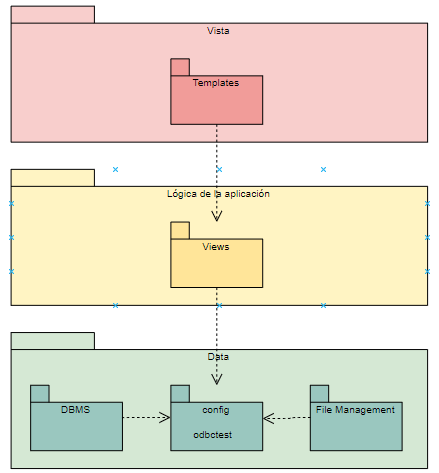
\includegraphics[scale=0.9]{DiagramaPaquetes}\newline

La vista, que es la parte de la interfaz se basa en los templates.\newline
Los templates dependen del fichero views, que es el que controla la lógica y envía los datos a los templates para mostrar unas u otras cosas y permitir distintos accesos por ejemplo.\newline
El views depende de los templates, que le pasan la información que introduce el usuario por pantalla y también depende de los datos recibidos de la base de datos y de los calendarios de Outlook.\newline
Las conexiones con el SGBD y con Outlook, a su vez, dependen del fichero odbctest y config respectivamente para poder establecer la conexión.

\apendice{Documentación técnica de programación}

\section{Introducción}
En esta sección describiré como está estructurado el proyecto, que es necesario para poder ejecutarlo desde cualquier ordenador y lo más relevante a la hora de crearlo.
\section{Estructura de directorios}
La estructura de los ficheros alojados en el \href{https://github.com/jgo0038/TFG-Reserva-aulas-informatica}{repositorio de GitHub} es la siguiente:
\begin{itemize}
    \item \textbf{ReservaAulas:} Contiene el proyecto y el entorno virtual y configuraciones.
    \begin{itemize}
        \item \textbf{.vscode:} Contiene la configuración para ejecutar en \textit{debug} desde \textit{VSCode}.
        \item \textbf{azureEnv:} Entorno virtual creado para el proyecto.
        \item \textbf{reservaAulas\_app:} Contiene el proyecto principal. Dentro se encuentran los ficheros que contienen la funcionalidad del proyecto. También alberga las conexiones con la base de datos, con Azure y con la API.
        \begin{itemize}
            \item \textbf{static:} Contiene imágenes, bibliotecas y ficheros javascript que se usan en el proyecto.
            \begin{itemize}
                \item \textbf{css:} Estilos de Bootstrap y algunos propios para HTML.
                \item \textbf{img:} Imágenes del proyecto.
                \item \textbf{js:} Ficheros JavaScript de Bootstrap.
            \end{itemize}
            \item \textbf{templates:} Contiene los ficheros de la parte de la vista del proyecto.
        \end{itemize}
        \item \textbf{requirements.txt:} Contiene los requisitos a instalar dentro del entorno virtual para el funcionamiento del proyecto.
        \item \textbf{startup:} Fichero para hacer el deploy a Azure.
    \end{itemize}
\end{itemize}
\section{Manual del programador}
\subsection{Estructura del proyecto}
En esta sección se explican las distintas entidades del proyecto y con qué finalidad se han creado. Se trata de explicar los ficheros del proyecto desde el punto de vista del programador para que se entienda el código para futuras mejoras o análisis del mismo. A continuación enumero y explico los ficheros usados:
\begin{itemize}
    \item \textbf{reservaAulas/azureEnv}: Entorno virtual creado para instalar las dependencias necesarias del proyecto.
    \item \textbf{reservaAulas/reservaAulas\_app}: Contiene todo el código del proyecto.
    \begin{itemize}
        \item \textbf{static}: Contiene las carpetas de 'css', 'img' y 'js'. En ellas se guardan los estilos de \textit{Bootstrap}, las imágenes que utilizamos y los archivos \textit{JavaScript} necesarios para \textit{Bootstrap} o alguno propio, respectivamente.
        \item \textbf{templates}: Contiene el código \textit{HTML}, \textit{Jinja2} y \textit{JavaScript} que crean las interfaces que verá el usuario.
        \item \textbf{reservaAulas\_app}: Contiene el código que maneja la lógica de la aplicación, proporciona y recoge los datos desde la API y base de datos.
    \end{itemize}
\end{itemize}

\begin{itemize}
    \item \textbf{reservaAulas/.deployment:} fichero generado al realizar el deploy en Azure.
    \item \textbf{log\_web\_app.log:} fichero generado para encontrar errores al hacer el deploy.
    \item \textbf{reservaAulas/createTablesSQLServer.sql:} fichero con el código correspondiente para generar las tablas y relaciones entre ellas necesarias para el proyecto.
    \item \label{requirements} \textbf{reservaAulas/requirements.txt:} fichero generado con las bibliotecas necesarias a instalar en el entorno virtual para que funcione la aplicación.
    \item \textbf{reservaAulas/startup.py:} fichero generado para ejecutar desde Azure.
    \item \textbf{reservaAulas/.vscode/launch.json:} configuración para ejecutar el proyecto desde el VSCode en un entorno virtual.
    \item \textbf{reservaAulas/reservaAulas\_app/\_\_init\_\_.py:} creación de la app de Flask e instancia de la base de datos y el cifrado csrf.
    \item \textbf{reservaAulas/reservaAulas\_app/config.py:} configuración de la aplicación con las claves iniciales de Azure para el uso de la API de Outlook y creación de los permisos.
    \item \textbf{reservaAulas/reservaAulas\_app/forms.py:} creación de los formularios que se utilizan en las páginas de la aplicación.
    \item \textbf{reservaAulas/reservaAulas\_app/getSQLData.py:} fichero con llamadas a la base de datos para ahorrar código en el fichero views.py.
    \item \textbf{reservaAulas/reservaAulas\_app/models.py:} modelos utilizados en base de datos en local.
    \item \textbf{reservaAulas/reservaAulas\_app/oauth\_helpers.py:} funciones que llaman a la API de Outlook para recoger, enviar, borrar o actualizar datos.
    \item \textbf{reservaAulas/reservaAulas\_app/odbctest:} conexión mediante pyodbc con la base de datos subida a Azure.
    \item \textbf{reservaAulas/reservaAulas\_app/views.py:} fichero que contiene la funcionalidad del servidor, llama a las funciones de otros ficheros para obtener datos y los envía al cliente.
    \item \textbf{reservaAulas/reservaAulas\_app/webapp.py:} fichero creado para la creación de la estructura pedida por VSCode y Azure.
    \item \textbf{reservaAulas/reservaAulas\_app/templates/anadirAulas.html:} fichero que contiene lo que verá el cliente a la hora de añadir un aula.
    \item \textbf{reservaAulas/reservaAulas\_app/templates/anadirPropietarios.html:} fichero que contiene la parte del cliente al intentar crear un propietario nuevo.
    \item \textbf{reservaAulas/reservaAulas\_app/templates/auditoria.html:} fichero que contiene el código para que el cliente pueda ver la tabla de auditorías.
    \item \textbf{reservaAulas/reservaAulas\_app/templates/errorModificarEvento.html:} fichero que permite al cliente ver el mensaje de error al intentar modificar un evento y que se solapen las horas con algún evento existente.
    \item \textbf{reservaAulas/reservaAulas\_app/templates/errorPermisos.html:} fichero que muestra al cliente un mensaje de error cuando se le ha hecho propietario de un calendario pero no se le han dado los permisos manualmente y no puede acceder a sus funcionalidades.
    \item \textbf{reservaAulas/reservaAulas\_app/templates/events.html:} página que pide al cliente las características de los eventos que se quieren visualizar .
    \item \textbf{reservaAulas/reservaAulas\_app/templates/eventsTable.html:} contiene el código de la parte del cliente que permite ver la tabla con los eventos que coincidan con las especificaciones pasadas, permite modificar y borrar los eventos si se tiene permisos.
    \item \textbf{reservaAulas/reservaAulas\_app/templates/home.html:} página de inicio de sesión y página principal si ya se ha iniciado sesión.
    \item \textbf{reservaAulas/reservaAulas\_app/templates/mensajePropietario.html:} fichero que permite al cliente ver el mensaje recordatorio al administrador para que asigne los permisos manualmente cuando crea un nuevo propietario o modifica el propietario de un aula.
    \item \textbf{reservaAulas/reservaAulas\_app/templates/navBar.html:} contiene código común para la barra de navegación superior y la franja inferior, heredan de ella para ahorrar código duplicado.
    \item \textbf{reservaAulas/reservaAulas\_app/templates/reservar.html:} fichero que contiene el código para mostrar al cliente la página desde la que pueden realizar una reserva de un aula.
    \item \textbf{reservaAulas/reservaAulas\_app/templates/showEventsTable.html:} contiene la tabla de eventos que se muestra al elegir la opción de ver los eventos de un aula que se va a reservar desde la ventana de reservar.
    \item \textbf{reservaAulas/reservaAulas\_app/templates/verAulas.html:} fichero que contiene el código que ve el cliente al ver la lista de aulas.
    \item \textbf{reservaAulas/reservaAulas\_app/templates/verPropietarios:} página que muestra una tabla en la que se ven los propietarios existentes.
\end{itemize}


\section{Compilación, instalación y ejecución del proyecto}
En esta sección será explicada la compilación, lo necesario para realizar la instalación correctamente y la forma de ejecutar el proyecto. Primeramente se explican los pasos que se tuvieron que realizar para poder registrar la aplicación en Microsoft Azure y permitir el acceso a el presente proyecto mediante el login de Microsoft que haremos funcionar al registrar la aplicación previamente.\newline

Comentando el uso de la API de Microsoft para acceder a los datos de Outlook y poder habilitar un inicio de sesión bajo Microsoft, hubo que registrar la aplicación en Azure Active Directory, para ello fueron seguidos estos pasos:
\begin{itemize}
    \item Acceder al centro de administración de Azure Active Directory.
    \item Acceder al apartado registro de aplicaciones y crear un nuevo registro.
    \item Una vez ahí dentro, se pedirá rellenar unos campos con el nombre de la aplicación, cuentas que accederán y lo más importante, la dirección URL de redirección al iniciar sesión mediante Outlook.\newline
    \imagen{AzureAutenticacion1}{URL de respuesta de nuestra aplicación}
    \item Una vez se ha creado, recogemos el ID de la aplicación obtenido, que se utilizará para obtener el secreto del cliente, que solamente se mostrará una vez y será necesario para el resto del proyecto. Para obtenerlo se accede a certificados y secretos, se escribe un nombre para registrar la aplicación y se elige una duración límite para que expire el secreto que se recibirá y haya que pedirlo de nuevo, de esta forma se obtiene dicho secreto desde Azure Active Directory.
\end{itemize}
Esto está especificado en el tutorial de Microsoft\cite{pythonMicrosoftGraph}. \newline
Una vez registrada la aplicación disponemos del código secreto, que no se volverá a repetir, y del identificador de la aplicación que se ve en la figura \ref{fig:AzureAutenticacion2}. Hubo que seguir una serie de pasos para incluirlo en el código y hacer que funcionara:
\imagen{AzureAutenticacion2}{Código de aplicación de Azure Active Directory}
\begin{itemize}
    \item Agregar al fichero 'config.py' el secreto recibido, el identificador de la aplicación de Azure y la ruta a la que redirigir una vez se ha logeado. Con esto se configura nuestro proyecto para la conexión con la aplicación registrada en Azure que se ha realizado en los pasos anteriores (ver figura \ref{fig:AzureAutenticacion}) .
    \imagen{AzureAutenticacion}{Código incluyendo la aplicación de Azure Active Directory}
    \item Agregar al fichero 'config.py' el código con los permisos de Outlook que se van a proporcionar al usuario que acceda, en este proyecto son los siguientes: leer el usuario, lectura de calendarios y calendarios compartidos, escritura de calendarios y calendarios compartidos, acceso al email, acceso offline,
    \item Crear en el ficheero 'oauth\_helpers.py' unas funciones con llamadas a la API REST para obtener un token de inicio de sesión y otro para refrescarle. Esto servirá para cada sesión de cada usuario diferente.
\end{itemize}
Una vez se creó este primer código que permitía acceder mediante el inicio de sesión de Outlook a la página que especificamos en Azure Active Directory como URL de redirección, se pudo empezar a trabajar con llamadas a la API REST para obtener información sobre los calendarios del usuario y sus eventos.\newline

La descarga del proyecto desde GitHub se puede realizar en:\newline
\url{https://github.com/jgo0038/TFG-Reserva-aulas-informatica}\newline
En el entorno de desarrollo, lo primero que hay que tener es una instalación de \textit{Python} y un entorno virtual, si no se tiene, habrá que crearlo de forma sencilla con el siguiente comando\newline
\textbf{\textit{python3 -m venv /path/to/new/virtual/environment}}\newline o utilizar directamente el que se descarga con el repositorio.
\newline
 Una vez se tenga esto creado, se activa el entorno virtual donde instalaremos las dependencias necesarias, como ya se explicó antes, especificadas en el fichero 'requirements.txt' (ver \ref{requirements}). Este fichero sirve para realizar una instalación muy simple con un sencillo comando: \newline
 \textbf{\textit{\$ pip install -r requirements.txt }} \newline
Con este comando se instalarán las bibliotecas necesarias para esta versión usada dentro de nuestro entorno virtual. El siguiente paso será la compilación y ejecución del proyecto. \newline

\label{ConexionDB}
Para la ejecución de nuestra aplicación web, se necesita un servidor web que haga de host para la base de datos. Como ya se ha visto en otros apartados, se ha utilizado Azure, por lo que la conexión con la base de datos ha sido particularizada para este servidor en concreto (ver fichero 'reservaAulas/reservaAulas\_app/odbctest.py') que contiene el nombre del servidor, de la base de datos, usuario, contraseña, puerto de Azure (1433) y driver para conectarse exactamente a esta base de datos de SQL Server alojada en Azure. Para que funcione con estas mismas configuraciones, hay que crear la base de datos con los mismos nombres que se muestran en la siguiente imagen, o bien adaptarlo a otra base de datos.\newline
\imagen{ConexionDBAzure1}{Código para conectar con la BD de Azure}
\newline Si se quisiera realizar en un servidor instalado en local, se tendría que cambiar la conexión y ajustarla al servidor utilizado. Azure restringe el acceso a las bases de datos desde otros ordenadores mediante la configuración del firewall, en el que se introducen las direcciones IP que pueden acceder a esta base de datos (actualmente solo puede realizarse desde el equipo utilizado por el alumno).\newline
\imagen{ConexionDBAzure2}{Restricción de direcciones IP para la conexión}
\newline
Debido a esta particularidad de la configuración del firewall de la base de datos, para poder acceder al proyecto como desarrollador se necesita crear una base de datos con las mismas relaciones que las especificadas en los diagramas y cambiar la conexión del fichero 'odbctest.py' para conectarse a ella, o bien añadir la IP al firewall de la base de datos de Azure.\newline
Si no se tiene acceso a la base de datos, se puede ejecutar desde el servidor de Azure al que está subida la aplicación accediendo desde el siguiente enlace \url{https://reservaaulas.azurewebsites.net} como cliente, esto lo veremos en el manual de usuario.\newline
Si se dispone de acceso a la base de datos, se podrá realizar una ejecución en local accediendo a la base de datos del servidor de Azure, para ello propongo dos opciones:\newline
Si se trabaja con VSCode (es el caso del alumno) los pasos a seguir son los siguientes:
\begin{itemize}
    \item Activar el entorno virtual.
    \item Ejecutar desde el modo debug que proporciona VSCode, ya está configurado en 'reservaAulas/.vscode/launch.json' el fichero que se tiene que ejecutar en el entorno para que el proyecto se ponga en marcha en el puerto elegido, que es el 5000.
    \item Acceder a la aplicación desde nuestro localhost.
\end{itemize}
Si por otro lado, se quiere ejecutar desde cualquier otro lugar, hay que establecer manualmente las configuraciones que se acaban de comentar. Esto se hace de la siguiente forma:
\begin{itemize}
    \item Activar el entorno virtual.
    \item Establecer la variable de entorno 'FLASK\_APP', el comando para hacerlo es el siguiente:\newline
    \textbf{\textit{\$ set FLASK\_APP=reservaAulas\_app.webapp}}\newline
    Si no utiliza Windows, use export en vez de set.
    \item El siguiente paso es ejecutar el proyecto, para ello ejecutamos la siguiente línea:\newline
    \textbf{\textit{python -m flask run}}
    \item Acceder a la aplicación desde nuestro localhost.
\end{itemize}
Una vez se tiene acceso a la aplicación, si la ejecutamos también logeados como el administrador necesitaremos acceder a Outlook para poder compartir los calendarios con los propietarios. A continuación dejo la serie de pasos a seguir para compartir manualmente un calendario con un responsable:
\begin{itemize}
    \item Iniciar sesión con la cuenta administrador del proyecto (las credenciales se facilitan en el archivo de texto 'EnlacesInteres.txt' adjunto al proyecto ).
    \item Acceder a la pestaña de calendarios de Outlook. \newline
   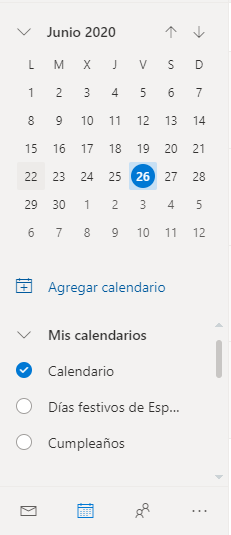
\includegraphics[scale=0.8]{CompartirCalendario}{Pestaña de calendarios}
    \item Pinchar en los tres puntos del calendario a compartir y elegir la opción de 'Uso compartido y permisos'.\newline
    \imagen{CompartirCalendario2}{Uso compartido y permisos}
    \item Escribir la dirección de correo del propietario con el que se quiere compartir el calendario, o seleccionar el icono de la papelera en el caso de querer quitar el permiso a algún propietario.\newline
    \imagen{CompartirCalendario3}{Compartir o borrar}
\end{itemize}
\section{Pruebas del sistema}
En esta sección realizaré pruebas manuales de los casos de uso sobre el sistema comprobando que todo funciona correctamente.
\tablaSmallSinColores{Pruebas manuales propietario}{p{7cm} p{7cm} }{pruebasmanuales}{
  \multicolumn{1}{p{3.25cm}}{\textbf{Descripción}} & \textbf{Respuesta{}}\\
 }
 {
  Iniciar sesión introduciendo los datos de una cuenta de Outlook  & {Se accede a la aplicación}\\\hline
  Consultar eventos de aulas &{Se muestra la tabla con los eventos que coincidan con las especificaciones.}\\\hline
  Consultar eventos de aulas sin completar los campos obligatorios & {Se pide que se rellenen los campos vacíos que sean obligatorios.}\\\hline
  Modificar un evento & {Se vuelve a la pantalla anterior y se muestra un mensaje de éxito en la modificación. Se modifica la información en el evento del calendario correspondiente de Outlook también.}\\\hline
  Modificar un evento cambiando la hora a unas ya ocupadas & {Se muestra una pantalla con un mensaje indicando que las horas están ocupadas y se ofrece la posibilidad de volver atrás.}\\\hline
  Borrar más de un evento seleccionado y aceptando la confirmación de los deseados & {Se muestra un mensaje de éxito en un cuadro de diálogo y se pide confirmación para mantenerse en la misma página con los mismos datos. Se borran los eventos de los calendarios de Outlook también.}\\\hline
  Realizar reserva introduciendo todos los campos correctamente y en fechas que estén libres & {Se queda en la misma página con el mismo formulario relleno que acabas de reservar y un mensaje en la parte inferior de éxito en la reserva. Se crea el evento en el calendario correspondiente de Outlook y se envía un email de notificación al profesor que solicitó la reserva.}\\\hline
  Realizar reserva introduciendo algún campo en blanco  & {Se pide que se rellenen los campos vacíos.}\\\hline
  Realizar reserva introduciendo fechas ya reservadas  & {Se queda en la misma página con el mismo formulario relleno que acabas de reservar y un mensaje en la parte inferior de error en las horas de la reserva.}\\\hline
  Consultar aulas especificando el edificio del que se quieren ver & {Se muestra una tabla con las aulas del edificio seleccionado y sus características.}

  }
 En esta tabla realizaré pruebas con funcionalidades únicamente del administrador.
 \tablaSmallSinColores{Pruebas manuales administrador}{p{7cm} p{7cm} }{pruebasmanuales}{
  \multicolumn{1}{p{3.25cm}}{\textbf{Descripción}} & \textbf{Respuesta{}}\\
 }
 {
  Modificar aulas & {Se vuelve a la página anterior y se muestra un mensaje por pantalla de éxito en la modificación.}\\\hline
  Modificar aulas cambiando el propietario & {Se muestra una pantalla en la que se lee un mensaje recordando al administrador de dar enviar el permiso de editar el calendario manualmente desde Outlook.}\\\hline
  Borrar un aula aceptando la confirmación & {Salta un cuadro de diálogo en el que se indica que se ha borrado correctamente el aula y se vuelve a la página anterior.}\\\hline
  Crear un aula con espacios en blanco en el formulario & {Se pide rellenar los espacios vacíos dejados.}\\\hline
  Crear un aula correctamente & {Se mantiene en la misma página mostrando el formulario completo y un mensaje en la parte inferior de éxito al crear el aula.}\\\hline
  Añadir un propietario sin completar todos los campos &
  {Se pide que se rellenen los campos vacíos}\\\hline
  }
\apendice{Documentación de usuario}

\section{Introducción}
En este apartado se explican los pasos a seguir por un usuario que quiere descargarse y utilizar la aplicación.
\section{Requisitos de usuarios}
Para poder utilizar la aplicación, el usuario tendrá que tener instalado Python. 
\section{Instalación}
Los pasos de la instalación para la ejecución de la aplicación son los mismos que se han explicado en el manual del programador. A continuación se explican las formas en las que se puede acceder al proyecto.\newline
Para el acceso de un usuario a la aplicación web, solamente necesita acceder al enlace en el que está subida dicha aplicación en Azure:\newline
\url{https://reservaaulas.azurewebsites.net}.
\newline
Lo único que se necesita es que el \textit{app service} en el que está realizado el deploy este ejecutándose y la base de datos de Azure activa. Estas acciones se explican a continuación:\newline
\begin{itemize}
    \item Acceder a \url{https://portal.azure.com/#home} con la cuenta  desde la que se registraron los servicios. Se muestra una página como la siguiente:\newline
    \imagen{ActivarServicios1}{Página portal de Azure.}
    \item Entrar en el app service llamado 'reservaAulas' y pinchar en el botón de la parte superior de 'Activar' o de 'reiniciar'.\newline
    \imagen{ActivarServicios2}{Activar app service}
    \item La base de datos se mantiene siempre activa para poder trabajar con la aplicación sin problemas.
\end{itemize}
Una vez se han seguido esos pasos, se asegura que el proyecto funcione ejecutándose desde la URL (https://reservaaulas.azurewebsites.net).
Para que esto funcione, fue necesario realizar un despliegue en un servicio de aplicación de Azure que se explica a continuación:\newline
\begin{itemize}
    \item Lo primero que se necesita es una suscripción a Azure, en mi caso utilicé la suscripción de estudiante, que me proporcionaba 100USD para realizar pruebas, aunque se agotaría el saldo y hubo que cambiar de plan de coste.
    \item Se necesita también un entorno de Python.
    \item Una vez tenemos los primeros requisitos, hay que crear un fichero 'requirements.txt' en el que se guarden las dependencias de la aplicación.
    \item Crear una instancia de un app service en Azure.
    \item Establecemos el comando de inicio al que nos indica Azure para el funcionamiento, almacenado en 'startup.txt' que es el siguiente:\newline \textit{\textbf{gunicorn --bind=0.0.0.0 --timeout 600 startup:app}}
    \item Realizar el despliegue, en el caso de este proyecto se hizo desde VSCode, mediante la extensión de 'Azure: app service'. Para esto, se inició sesión con Azure en dicha extensión, ahí se muestran los app services dónde se puede realizar el despliegue y se selecciona el creado anteriormente.
\end{itemize}
Esta explicación se puede ver más detallada en el manual proporcionado por Microsoft del siguiente enlace \cite{deployVSCode}.\newline
Como se puede ver se crean los ficheros y la estructura según pide Microsoft y VSCode a lo largo del proyecto, por lo que el proyecto está creado para ser ejecutado en este entorno y servidor.


\section{Manual del usuario}
A continuación se explicará como realizar las operaciones que proporciona esta aplicación:
\subsection{Inicio de la aplicación}
Para comenzar a utilizar la aplicación se puede hacer de dos formas:
\begin{itemize}
    \item Sin inicio de sesión (como invitado) que puede ver las reservas realizadas sobre las aulas y las aulas existentes. Para ello, hay que pinchar en el botón de 'Comience a usar la app' de la página principal (ver figura \ref{fig:InicioSesion1}).
    \item Iniciando sesión con Outlook. Pinchando sobre el botón de 'Iniciar sesión desde Outlook' e introduciendo los datos de una cuenta de Microsoft (ver figura \ref{fig:InicioSesion1}).
\end{itemize}
\imagen{InicioSesion1}{Página principal.}
\subsection{Consultar ocupación de aulas}
Pasos para consultar la ocupación de un aula:
\begin{itemize}
    \item Pinchar en el botón de 'Consultar ocupación de aulas'
    \item Escoger el edificio en el que se encuentra el aula que se quiere comprobar(ver figura \ref{fig:ConsultarEventos1}).
    \item Se muestra un formulario en el que aparecen dos opciones (ver figura \ref{fig:ConsultarEventos2}):
    \begin{itemize}
        \item Seleccionar un aula y rellenar al menos los campos obligatorios para filtrar las horas y fechas de las reservas a mostrar de ese aula.
        \item Seleccionar 'Cualquiera' en la opción del aula y rellenar al menos los campos obligatorios. Esto filtrará todas las aulas de ese edificio según las fechas especificadas. Además se pueden rellenar los campos opcionales de 'Capacidad', 'Numero de ordenadores' o 'Tipo' para filtrar las aulas según esas características.
    \end{itemize}
    \item Pinchar en el botón 'Enviar consulta' y se mostrarán los eventos que coincidan en una tabla (ver figura \ref{fig:ConsultarEventos3}).
\end{itemize}
\imagen{ConsultarEventos1}{Página inicial para ver eventos de aulas.}
\imagen{ConsultarEventos2}{Formulario para consultar eventos.}
\imagen{ConsultarEventos3}{Tabla donde se muestran los eventos.}

\subsection{Modificar eventos}
Para modificar eventos, es necesario acceder previamente a la página de la consulta de eventos que se ha explicado en la sección anterior, una vez ahí:
\begin{itemize}
    \item Se pulsa en el botón 'Modificar' de la parte derecha de la tabla (ver figura \ref{fig:ModificarEventos1}).
    \item Se abre un formulario en la parte superior de la página en la que se muestran los datos del evento seleccionado y se puede modificar. Una vez modificado si se pincha en 'Modificar' se guardan los cambios (ver figura \ref{fig:ModificarEventos2}).
\end{itemize}
\imagen{ModificarEventos1}{Página inicial para ver eventos de aulas y modificarlos.}
\imagen{ModificarEventos2}{Formulario para modificar eventos.}

\subsection{Borrar eventos}
Para borrar eventos, hay que acceder primero a la página de la consulta de eventos que se ha explicado anteriormente, una vez ahí:
\begin{itemize}
    \item Se pula en el botón 'Seleccione para borrar' de la parte derecha de la tabla de los eventos que se quieren borrar (ver figura \ref{fig:ModificarEventos1}).
    \item Se resaltan en rojo estos eventos seleccionados (ver figura \ref{fig:BorrarEventos2}).
    \item Se pincha en el botón de la parte inferior de la página de 'Borrar eventos seleccionados' y sale un cuadro de diálogo en el que se pide la confirmación para borrar (ver figura \ref{fig:BorrarEventos3}). Si se acepta, se borran los eventos seleccionados.
\end{itemize}
\imagen{ModificarEventos1}{Página inicial para ver eventos de aulas y borrarlos.}
\imagen{BorrarEventos2}{Selección de eventos a borrar.}
\imagen{BorrarEventos3}{Confirmación de borrado.}

\subsection{Realizar reserva}
Pasos a seguir para realizar la reserva de un aula:
\begin{itemize}
    \item Seleccionar en el formulario de la izquierda los valores deseados y pinchar en el botón 'Consultar' (ver figura \ref{fig:Reservar1}). Esto rellena la columna de la derecha el desplegable de 'Selecciona aula'.
    \item Elegir un tipo de reserva y pinchar en 'Aplicar'. Varía el número de campos a rellenar.
    \item Completar la información pedida sobre la reserva en la parte derecha (ver figura \ref{fig:Reservar2}).
\end{itemize}
\imagen{Reservar1}{Pantalla inicial de la reserva.}
\imagen{Reservar2}{Pantalla completa antes de la reserva.}

\subsection{Modificar aulas}
Pasos a seguir para realizar la modificación de un aula:
\begin{itemize}
    \item Acceder a la ventana de 'Ver/modificar aulas'.
    \item Seleccionar un grupo de aulas en el que estará el aula que queremos modificar. Se mostrará una tabla con todas las aulas de dicho grupo (ver figura \ref{fig:Modificar1}).
    \item Seleccionar el botón 'Editar', se abrirá un formulario en la parte superior para poder editar los datos del aula. Una vez editados pinchar en el botón 'Guardar'. (ver figura \ref{fig:Modificar2}).
\end{itemize}
\imagen{Modificar1}{Pantalla inicial de la modificación.}
\imagen{Modificar2}{Pantalla completa antes de la modificación.}

\subsection{Añadir aulas}
Pasos a seguir para añadir un aula:
\begin{itemize}
    \item Acceder a la ventana de 'Añadir aulas'.
    \item Rellenar el formulario que se presenta indicando los datos pedidos. Pinchar en 'crear aula'.
    \imagen{AñadirAulas}{Pantalla para añadir un aula.}
    \item Una vez se ha añadido el aula, se accede a los calendarios de Outlook y se asignan los permisos manualmente al responsable correspondiente de este nuevo aula.
\end{itemize}

\subsection{Ver auditorías}
Para ver la tabla de las auditorías, que muestra los cambios realizados sobre las reservas de todos los calendarios, hay que ser administrador y pinchar en el botón de 'Ver auditorías'.
\imagen{Auditorias}{Pantalla para ver la tabla de auditorías.}

\subsection{Modificar propietario}
Pasos a seguir para modificar un propietario:
\begin{itemize}
    \item Acceder a la ventana de 'Ver propietarios'.
    \item Se muestra una tabla con los propietarios existentes y un botón de 'Editar' a su derecha (ver figura \ref{fig:ModificarPropietario1}).
    \item Aparecerá un formulario en la parte superior de la página con los datos del propietario a editar, ahí se podrá modificar y pinchar en el botón 'Modificar' para guardar los cambios (ver figura \ref{fig:ModificarPropietario2}).

    \imagen{ModificarPropietario1}{Pantalla inicial de la modificación de propietario.}
    \imagen{ModificarPropietario2}{Pantalla completa antes de la modificación.}
    \item Una vez se ha modificado el propietario, si se ha cambiado el responsable, se accede a los calendarios de Outlook y se asignan los permisos manualmente al responsable correspondiente después de la modificación.
\end{itemize}


\bibliographystyle{plain}
\bibliography{bibliografiaAnexos}

\end{document}
